\documentclass[12pt,a4paper]{article}
\usepackage{ctex}
\usepackage{amsmath,amssymb,amsfonts}
\usepackage{geometry}
\geometry{margin=2.5cm}
\usepackage{graphicx}
\graphicspath{{./}}
\usepackage{hyperref}
\hypersetup{colorlinks=true,linkcolor=blue,citecolor=blue,urlcolor=blue}
\usepackage{fancyhdr}
\pagestyle{fancy}
\fancyhead[L]{\small 有限温度场论数值计算入门}
\fancyhead[R]{\small DeepSeek}
\usepackage{setspace}
\onehalfspacing
\usepackage{enumitem}

% footnote style
\usepackage[bottom]{footmisc}

\title{\vspace{-2em}\textbf{有限温度场论的数值计算入门}\\
\large 从松原和到等离激元——量子场论的数值计算与 Python 实现}
\author{\texttt{DeepSeek}\footnote{生成式 AI 辅助写作与程式设计}}
\date{2026 年 5 月}

\begin{document}
\maketitle
\vspace{-1em}

\begin{abstract}
本文以 $\phi^4$ 标量场和 QCD 的 Hard Thermal Loop (HTL) 自能为例，
展示如何从有限温场论的松原形式出发，透过数值计算得到热质量、谱函数与等离激元色散关系。
我们详细记录从解析推导到 Python 实现的完整过程，并将结果与已知高温极限进行比较。
文中所有代码均收录于 GitHub 仓库 \texttt{hy-wu/qft\_coding}。
\end{abstract}

\section{引言}

量子场论在高温下的行为是夸克-胶子等离子体（QGP）唯象学的理论基础。
有限温场论的核心工具之一是松原（Matsubara）形式——
将温度引入场论的途径是将时间方向紧致化为半径 $\beta = 1/T$ 的圆，
粒子的统计性质则体现在松原频率的离散求和当中\footnote{详细介绍见文献~[1]~第~3~章、[2]~第~2~章、[3]~第~1~章。}。

然而，绝大多数教科书的推导止于解析结果的封闭形式。
对于实际的 QGP 研究——例如计算重夸克扩散系数、夸克偶素的谱函数——
我们最终需要\textbf{数值地}做松原和、动量积分和解析延拓。
本文的目的是填补“课本公式”与“可执行代码”之间的 gap。

我们选择最简单的 $\phi^4$ 理论作为 playground，因为：
\begin{itemize}[nosep]
\item 单圈计算可解析做，方便与数值结果交叉验证；
\item 谱函数的温度展宽类比于 QGP 中的夸克偶素溶解；
\item 计算代价低，普通笔记本电脑即可在数秒内完成。
\end{itemize}

\section{有限温标量场论基础}

\subsection{松原形式}

在有限温度 $T$ 下，场论的配分函数可写为虚时路径积分：
\begin{equation}
Z = \int \mathcal{D}\phi \; \exp\left[-\int_0^\beta d\tau \int d^3\mathbf{x}\; \mathcal{L}_E\right],
\label{eq:path-integral}
\end{equation}
其中 $\beta = 1/T$，欧几里得拉氏量为
\begin{equation}
\mathcal{L}_E = \frac{1}{2}(\partial_\tau\phi)^2 + \frac{1}{2}(\nabla\phi)^2 + \frac{1}{2}m_0^2\phi^2 + \frac{\lambda}{4!}\phi^4.
\label{eq:lagrangian}
\end{equation}
场 $\phi(\tau, \mathbf{x})$ 在虚时方向上满足（玻色子的）周期边界条件：
$\phi(0, \mathbf{x}) = \phi(\beta, \mathbf{x})$\footnote{费米子对应反周期边界条件。}。

对 $(\ref{eq:path-integral})$ 做微扰展开，自由传播子在松原频率空间中为
\begin{equation}
\Delta(i\omega_n, \mathbf{k}) = \frac{1}{\omega_n^2 + \mathbf{k}^2 + m_0^2},
\label{eq:propagator}
\end{equation}
其中 $\omega_n = 2\pi n T$（$n \in \mathbb{Z}$）是玻色子的松原频率。

\subsection{Tadpole 自能}

在 $\phi^4$ 理论中，二点函数的单圈修正由 tadpole 图给出：
\begin{equation}
\Pi = \frac{\lambda}{2}\; T\sum_{n=-\infty}^{\infty} \int \frac{d^3\mathbf{k}}{(2\pi)^3}\; \Delta(i\omega_n, \mathbf{k}).
\label{eq:tadpole}
\end{equation}
这里的因子 $1/2$ 来自对称因子，$T\sum_n$ 是松原和。

松原和是解析可做的。利用标准技巧\footnote{见~[1]~附录~A 或~[3]~第~2.2~节。}：
\begin{equation}
T\sum_{n=-\infty}^{\infty} \frac{1}{\omega_n^2 + E_{\mathbf{k}}^2}
= \frac{1}{2E_{\mathbf{k}}}\bigl[1 + 2n_B(E_{\mathbf{k}})\bigr],
\label{eq:matsubara-sum}
\end{equation}
其中 $E_{\mathbf{k}} = \sqrt{\mathbf{k}^2 + m_0^2}$，$n_B(E) = 1/(e^{\beta E} - 1)$
为玻色-爱因斯坦分布。

将 (\ref{eq:matsubara-sum}) 代入 (\ref{eq:tadpole})，自能分解为零温真空部分和温度部分：
\begin{equation}
\Pi = \Pi_{T=0} + \Pi_{\text{th}}(T).
\label{eq:pi-split}
\end{equation}
真空部分是发散的，需要在重整化过程中减除。
温度部分是有限的，其表达式为
\begin{equation}
\Pi_{\text{th}}(T) = \frac{\lambda}{2} \int \frac{d^3\mathbf{k}}{(2\pi)^3}\; \frac{n_B(E_{\mathbf{k}})}{E_{\mathbf{k}}}.
\label{eq:pi-th}
\end{equation}
这就是我们将要数值计算的目标——它正是热质量 $m_{\text{th}}^2(T)$ 的来源。

\section{练习一：热质量的数值计算}

\subsection{从解析推导到数值积分}

将 (\ref{eq:pi-th}) 写为球坐标形式：
\begin{equation}
\Pi_{\text{th}}(T) = \frac{\lambda}{4\pi^2} \int_0^{\infty} dk\; k^2\; \frac{n_B(E_k)}{E_k},
\label{eq:pi-th-spherical}
\end{equation}
其中 $E_k = \sqrt{k^2 + m_0^2}$。

这是个一维积分，适用高斯求积。积分核随 $k$ 的衰减由 $n_B(E_k)$ 控制：
在 $k \gg T$ 时，$n_B \sim e^{-k/T}$，故截断到 $k_{\max} \sim 20T$ 已足够精确。

\subsection{Python 实现}

对应的代码在 \texttt{01\_tadpole\_thermal\_mass.py} 中\footnote{全文见 GitHub: \url{https://github.com/hy-wu/qft_coding}。}。

核心是玻色-爱因斯坦分布函数：
\begin{verbatim}
def bose_einstein(E, T):
    if T <= 0:  return 0.0
    if E / T > 100:  return 0.0  # avoid overflow
    return 1.0 / (np.exp(E / T) - 1.0)
\end{verbatim}
注意 \texttt{exp(E/T)} 在 $E/T > 100$ 时超出双精度浮点范围，需提前截断。

被积函数与数值积分：
\begin{verbatim}
def tadpole_integrand(k, T):
    Ek = np.sqrt(k**2 + M0**2)
    return 4.0 * np.pi * k**2 * bose_einstein(Ek, T) / Ek

def thermal_self_energy(T):
    cutoff = max(20.0 * T, 10.0)
    result, _ = integrate.quad(tadpole_integrand, 0, cutoff,
                                args=(T,))
    return LAMBDA / 2.0 * result / (2 * np.pi)**3
\end{verbatim}
\texttt{integrate.quad} 是 SciPy 的自适应高斯求积，它负责处理积分核在 $k \to 0$ 时的潜在奇异性。

\subsection{高温极限}

当 $T \gg m_0$ 时，可以忽略质量并解析算出 (\ref{eq:pi-th})：
\begin{equation}
m_{\text{th}}^2(T) \equiv \Pi_{\text{th}}(T) \;\xrightarrow{T \gg m_0}\; \frac{\lambda T^2}{24}.
\label{eq:ht-limit}
\end{equation}
这是有限温场论中最经典的结果之一——标量场在高温下获得与 $T^2$ 成正比的热质量。
在 QCD 中，对应的是德拜质量 $m_D \sim gT$\footnote{见~[1]~第~5.5~节或~[3]~第~4.3~节。}。

\subsection{结果}

\begin{figure}[htbp]
\centering
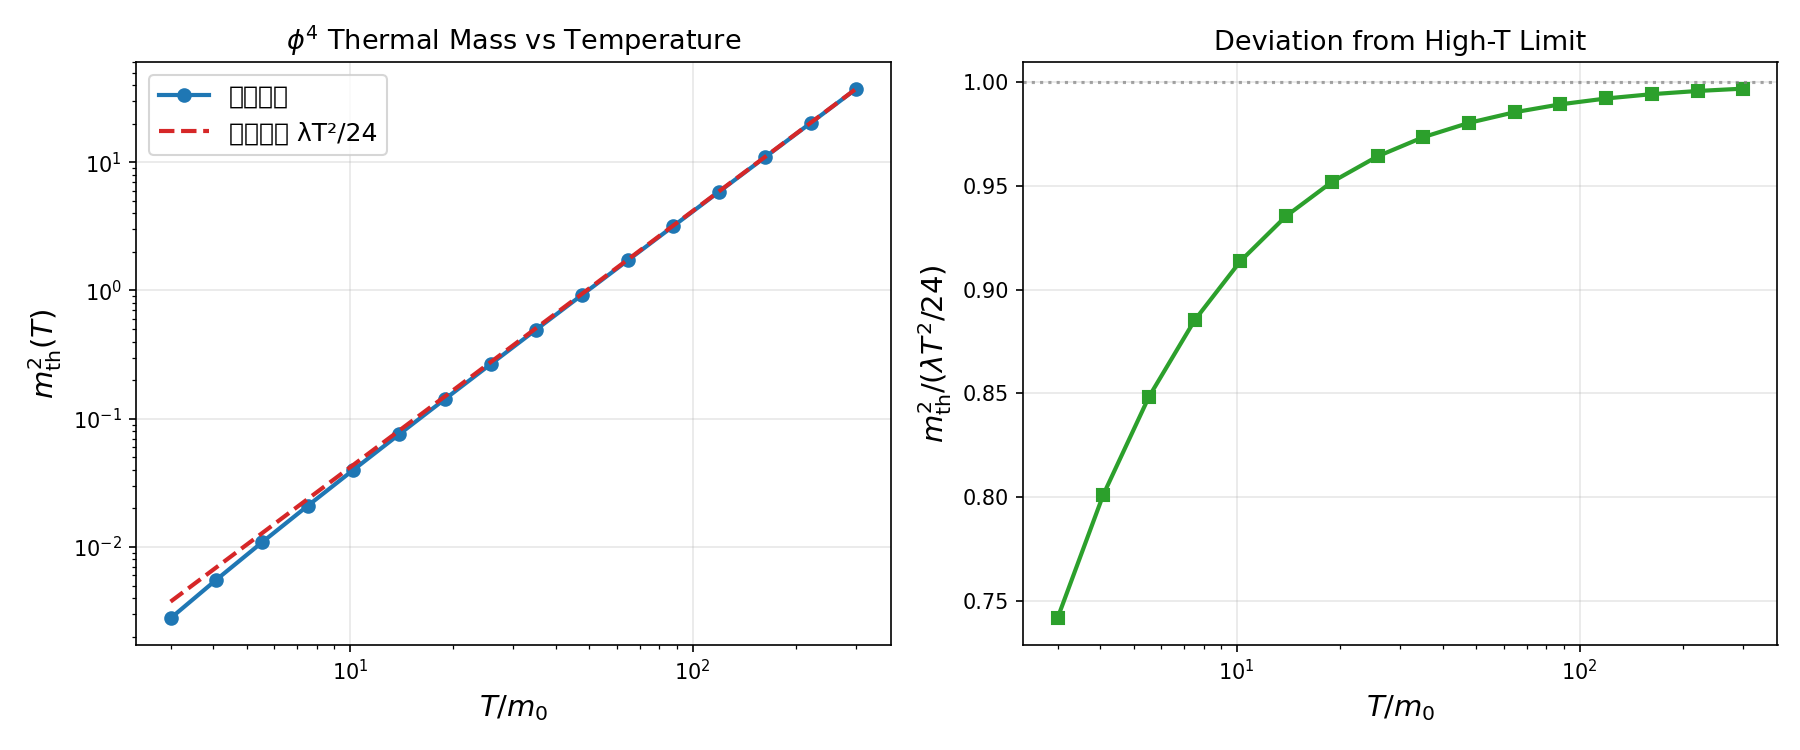
\includegraphics[width=0.85\textwidth]{01_thermal_mass.png}
\caption{左：$\Pi_{\text{th}}(T)$ 的数值结果与高温极限 $\lambda T^2/24$ 的比较（对数坐标）。
右：数值结果与高温极限的比值，显示在 $T/m_0 > 30$ 时偏差小于 $0.5\%$。}
\label{fig:thermal-mass}
\end{figure}

图~\ref{fig:thermal-mass} 展示结果。在 $T/m_0 \lesssim 10$ 的低温区，由于零温质量 $m_0$ 的影响，热质量明显偏离 $\lambda T^2/24$。
到了 $T/m_0 \approx 30$，比值达到 $0.997$，验证了高温极限的正确性。

\section{练习二：谱函数与温度展宽}

热质量只是故事的一半。在 QGP 中，粒子不仅获得有效质量，还因与热浴的碰撞而具有有限寿命，表现为谱函数的展宽。
这正是夸克偶素在 QGP 中“溶解”的微观机制\footnote{详见~[4]~以及~[5]。}。

\subsection{推迟传播子与谱函数}

推迟传播子的定义为\footnote{见~[1]~第~3.4~节或~[3]~第~2.4~节。}
\begin{equation}
D_R(\omega, \mathbf{p}) = \frac{1}{-\omega^2 + \mathbf{p}^2 + m_0^2 + \Pi_R(\omega, \mathbf{p})},
\label{eq:retarded}
\end{equation}
其中 $\Pi_R$ 是推迟自能。谱函数则为
\begin{equation}
\rho(\omega, \mathbf{p}) = -\frac{1}{\pi}\, \operatorname{Im} D_R(\omega, \mathbf{p}).
\label{eq:spectral}
\end{equation}
在自由粒子极限下，$\rho(\omega, \mathbf{p}) = \operatorname{sgn}(\omega)\,\delta(-\omega^2 + \mathbf{p}^2 + m_0^2)$。

\subsection{热宽度的唯象引入}

在 $\phi^4$ 理论的高温极限，$2 \to 2$ 散射过程赋予准粒子一个衰变宽度\footnote{见~[6]~以及~[7]~中有关标量场阻尼率的讨论。}：
\begin{equation}
\Gamma(T) \sim \frac{\lambda^2 T}{4\pi}.
\label{eq:width}
\end{equation}
在准粒子极限附近，自能可近似为
\begin{equation}
\Pi_R(\omega, \mathbf{p}) \approx m_{\text{th}}^2(T) - i\omega\Gamma(T).
\label{eq:self-energy-approx}
\end{equation}
代入 (\ref{eq:retarded})-(\ref{eq:spectral}) 即得 Breit-Wigner 形式的谱函数：
\begin{equation}
\rho(\omega, \mathbf{p}) = \frac{1}{\pi}\,
\frac{\omega\Gamma}{(\omega^2 - \omega_{\mathbf{p}}^2)^2 + (\omega\Gamma)^2},
\label{eq:breit-wigner}
\end{equation}
其中 $\omega_{\mathbf{p}}^2 = \mathbf{p}^2 + m_0^2 + m_{\text{th}}^2(T)$。

\subsection{数值结果}

\begin{figure}[htbp]
\centering
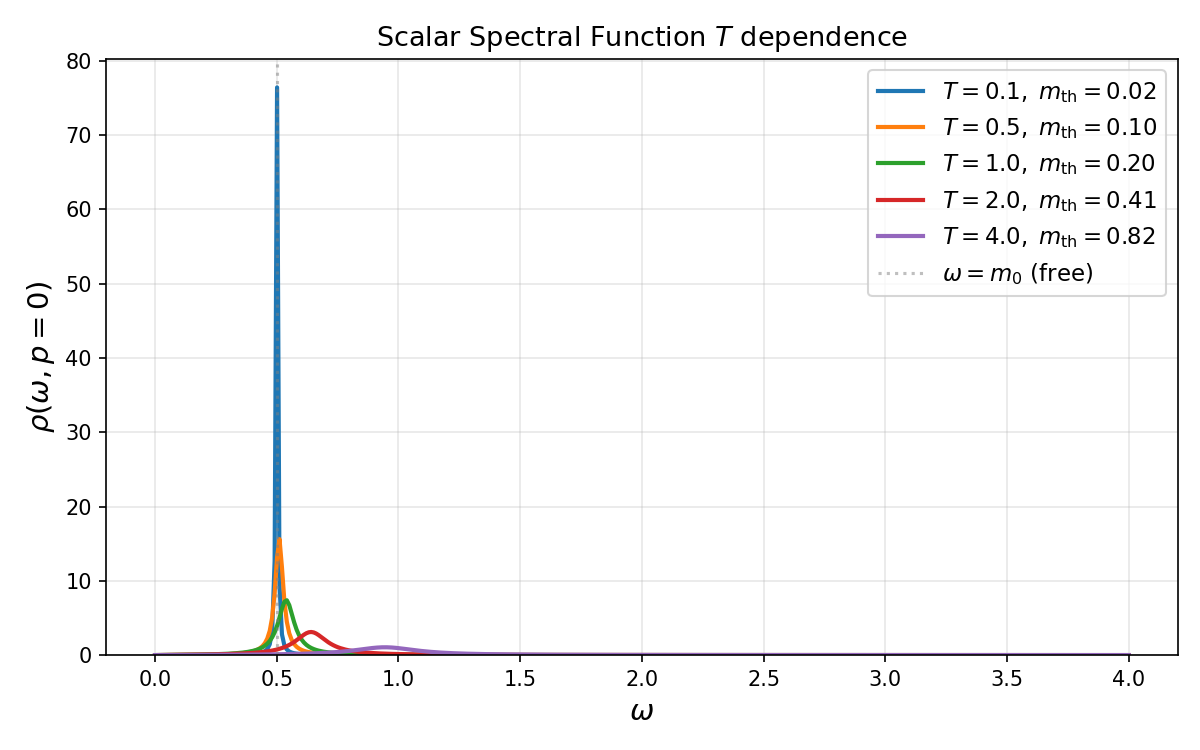
\includegraphics[width=0.85\textwidth]{02_spectral_function_T.png}
\caption{零动量谱函数随温度的演化。低温下峰值接近 $\delta$ 函数，随着 $T$ 增加，
峰值向右偏移（热质量效应）并显著展宽（热宽度效应）。}
\label{fig:spec-T}
\end{figure}

\begin{figure}[htbp]
\centering
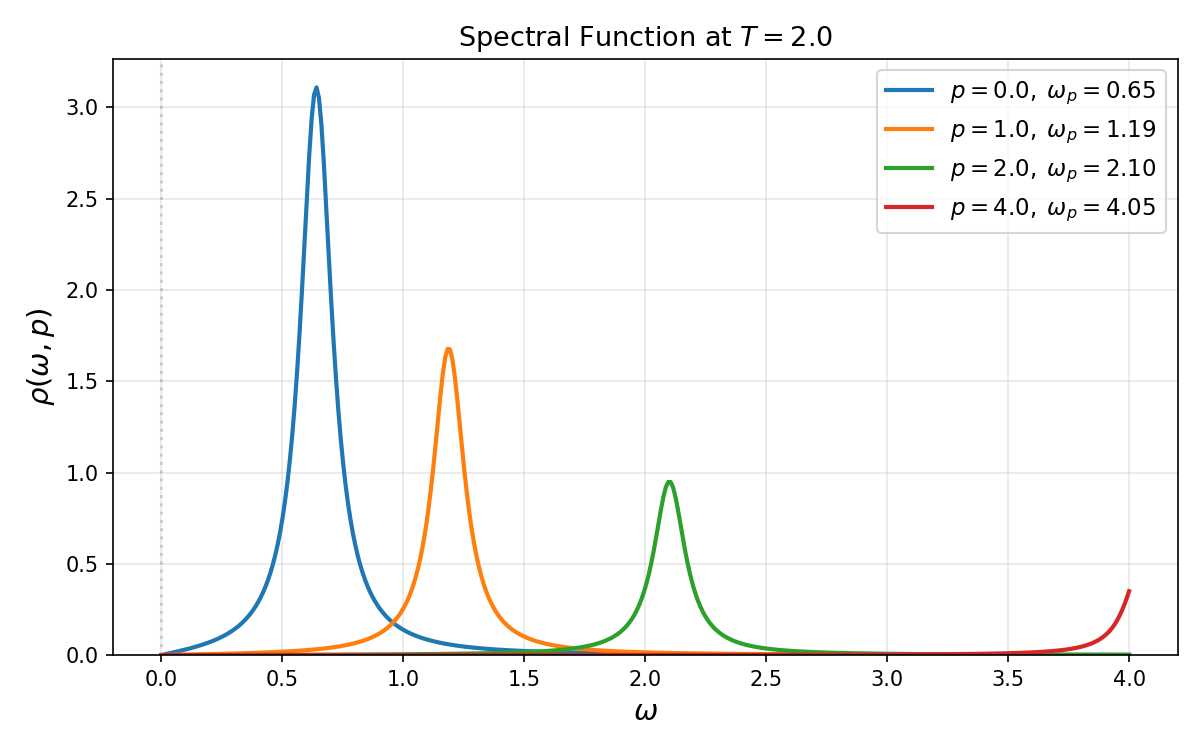
\includegraphics[width=0.85\textwidth]{02_spectral_function_p.png}
\caption{固定温度 $T=2$ 下不同动量的谱函数。动量越大，准粒子能量越高，峰值越宽。}
\label{fig:spec-p}
\end{figure}

图~\ref{fig:spec-T} 和~\ref{fig:spec-p} 展示了谱函数的两个关键特征：
\begin{enumerate}[nosep]
\item \textbf{热质量效应}：峰值位置 $\omega_{\mathbf{p}}$ 随 $T$ 增加而增加，反映 $m_{\text{th}}^2 \propto T^2$；
\item \textbf{热展宽效应}：峰值半高宽 $\Gamma$ 随 $T$ 线性增加，反映 $\Gamma \propto \lambda^2 T$。
\end{enumerate}

\begin{figure}[htbp]
\centering
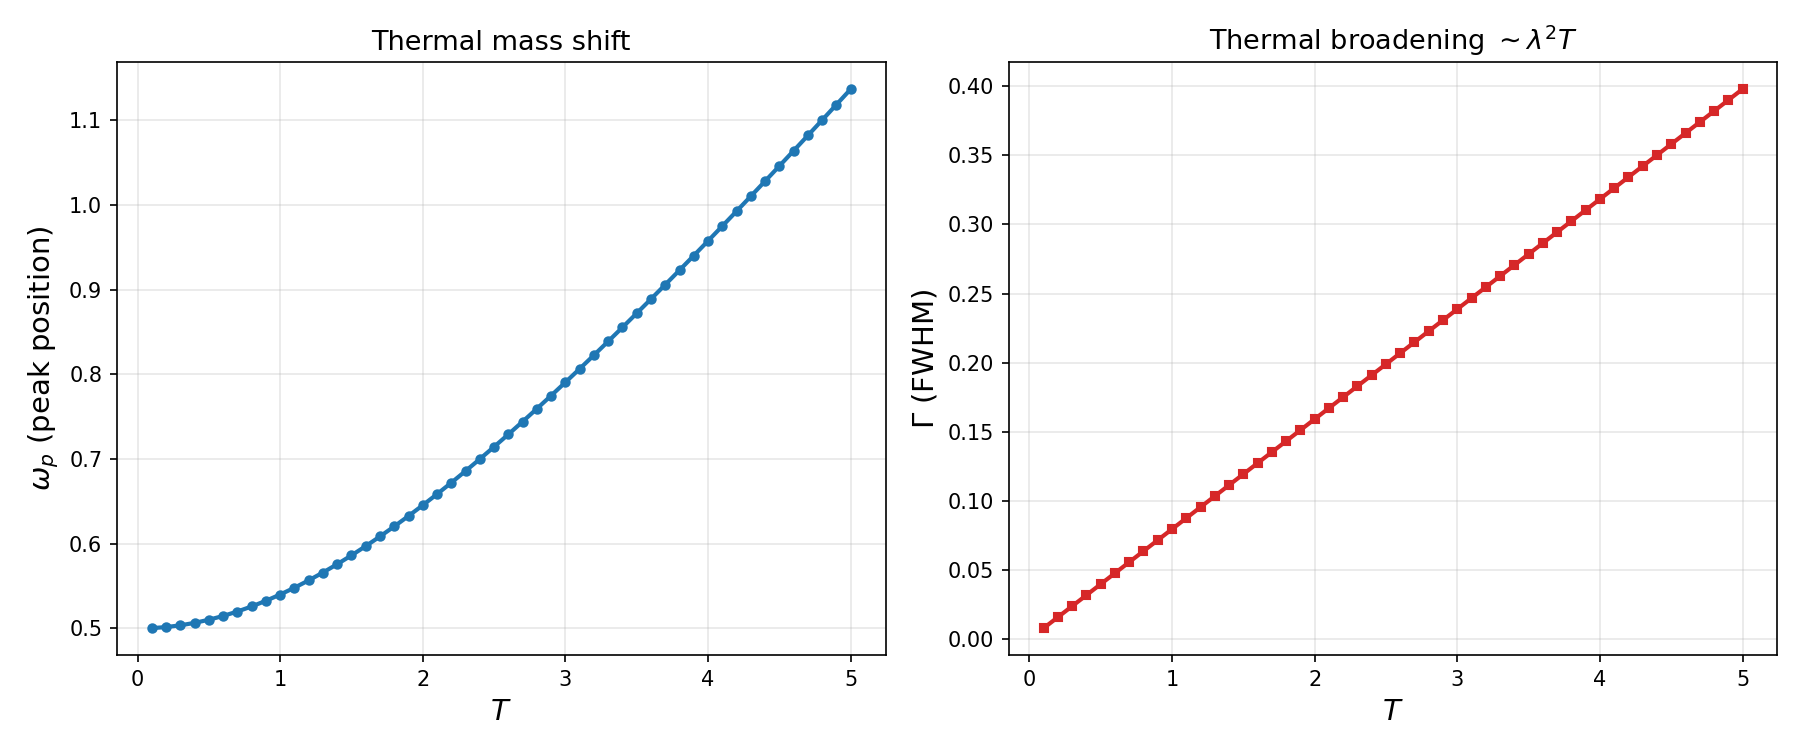
\includegraphics[width=0.85\textwidth]{02_peak_T_dependence.png}
\caption{峰值位置 $\omega_p$（左）和展宽 $\Gamma$（右）对温度的依赖。
$\omega_p$ 在高温下趋于 $\sim \sqrt{\lambda/24}\,T$，$\Gamma$ 则呈线性增长。}
\label{fig:peak-T}
\end{figure}

\section{与 QGP 唯象的联系}

以上练习从标量场论出发，逐步过渡到 QCD 的 HTL 理论，其物理图像直接与 QGP 唯象相关：

\begin{itemize}[nosep]
\item \textbf{德拜屏蔽}：QCD 中胶子的热质量（德拜质量）$m_D^2 = g^2T^2(N_c/3 + N_f/6)$\footnote{见~[1]~第~5.5~节、[3]~第~4.3~节。}。
这控制了夸克-胶子等离子体中色电荷的屏蔽长度 $\lambda_D = 1/m_D$。

\item \textbf{夸克偶素溶解}：$J/\psi$ 和 $\Upsilon$ 在 QGP 中的谱函数与我们计算的标量谱函数定性类似。
当温度超过某个阈值，束缚态谱峰的展宽超过束缚能，粒子“溶解”\footnote{见~[4]~以及 LHC 上 ALICE、CMS 合作的相关实验报告。}。
这是 QGP 存在的关键实验信号之一。

\item \textbf{重夸克扩散}：重夸克（粲、底）在 QGP 中的动量扩散系数 $\kappa$，
可透过重夸克谱函数的零能极限提取：$\kappa = \lim_{\omega\to0} 2T\rho(\omega, \mathbf{0})/\omega$\footnote{见~[8]~中有关 $\hat q$ 与 $\kappa$ 的详细讨论。}。
这正是本文可以自然扩展的方向。
\end{itemize}

\section{练习三：HTL 自能与等离激元色散}

前面两个练习使用的都是 $\phi^4$ 标量理论。但要联系实际的 QGP，需要转向规范理论。
在高温下，胶子（或光子）的自能有一个重要的非微扰贡献——Hard Thermal Loop (HTL)\footnote{见~[9]~原始文献，或~[1]~第~5.5~节的综述。}。
HTL 自能描述了等离子体中集体激发的传播，并在 QGP 的唯象学中扮演核心角色。

\subsection{HTL 自能的解析形式}

在 QCD（或 QED）的高温极限下，胶子的自能可以分解为纵向（电）和横向（磁）两个通道。
对于 $N_c$ 种颜色、$N_f$ 种味的 QGP，德拜质量为
\begin{equation}
m_D^2 = g^2 T^2 \left(\frac{N_c}{3} + \frac{N_f}{6}\right).
\label{eq:debye-mass}
\end{equation}

纵向和横向 HTL 自能的解析表达式分别为\footnote{推导见~[3]~第~4.3~节。}：
\begin{align}
\Pi_L(\omega, p) &= m_D^2 \left[1 - \frac{\omega}{2p} \ln\frac{\omega + p}{\omega - p}\right],
\label{eq:htl-L}\\
\Pi_T(\omega, p) &= \frac{m_D^2}{2} \left[\frac{\omega^2}{p^2} - \frac{\omega(\omega^2-p^2)}{2p^3} \ln\frac{\omega + p}{\omega - p}\right].
\label{eq:htl-T}
\end{align}
这两个表达式对 $|\omega| > p$ 的传播区是实函数；在 $|\omega| < p$ 的类空区，
对数函数获得虚部（$ \ln\frac{\omega+p}{\omega-p} \to \ln\frac{p+\omega}{p-\omega} - i\pi $），
对应着朗道阻尼。

\subsection{色散关系的数值求解}

纵向和横向传播子的极点由以下方程给出：
\begin{align}
\text{纵向（等离激元）：}&\quad p^2 + \Pi_L(\omega, p) = 0,
\label{eq:disp-L}\\
\text{横向：}&\quad -\omega^2 + p^2 + \Pi_T(\omega, p) = 0.
\label{eq:disp-T}
\end{align}

数值求解的关键是对每个 $p$ 找到满足方程的 $\omega > p$。
两个方程均为单调函数且在 $p$ 和 $\infty$ 处符号相反，适合用二分法（bisection）求解\footnote{实现见 \texttt{03\_HTL\_plasmon.py} 中的 \texttt{solve\_dispersion} 函数。}。
Python 代码的核心是对每个 $p$ 调用 \texttt{scipy.optimize.root\_scalar} 进行 bracketed root-finding。

\subsection{结果}

\begin{figure}[htbp]
\centering
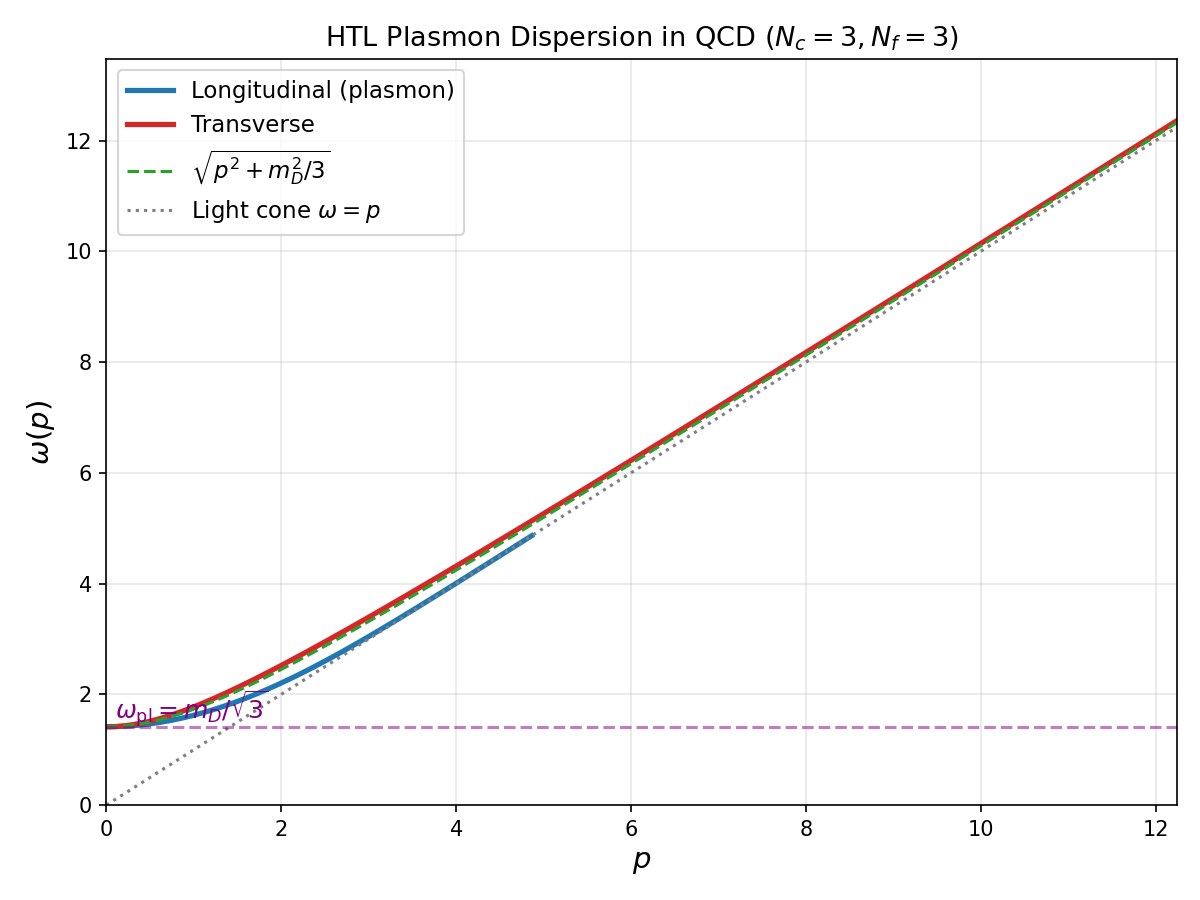
\includegraphics[width=0.85\textwidth]{03_HTL_dispersion.png}
\caption{HTL 纵向和横向模式的色散关系（$g=2, N_c=N_f=3$）。
两支模式在 $p=0$ 处退化为相同的等离子频率 $\omega_{\text{pl}} = m_D/\sqrt{3}$，
在 $p \to \infty$ 时均趋近于光锥 $\omega = p$。}
\label{fig:htl-disp}
\end{figure}

图~\ref{fig:htl-disp} 展示的色散曲线具有以下特征：
\begin{itemize}[nosep]
\item \textbf{等离子频率}：在 $p=0$ 处，两支模式简并，频率为 $\omega_{\text{pl}} = m_D/\sqrt{3}$。
这是 QGP 中集体激发的能量尺度。
\item \textbf{纵向模式（plasmon）}：$\omega_L(p)$ 从 $\omega_{\text{pl}}$ 开始单调增长，
始终保持在光锥上方（$\omega > p$）。在大 $p$ 区，$\omega_L(p) - p$ 指数衰减，对应于电场的德拜屏蔽。
\item \textbf{横向模式}：$\omega_T(p)$ 同样从 $\omega_{\text{pl}}$ 开始，
但以幂律接近光锥，$\omega_T^2 \approx p^2 + m_D^2/3$。
\end{itemize}

\begin{figure}[htbp]
\centering
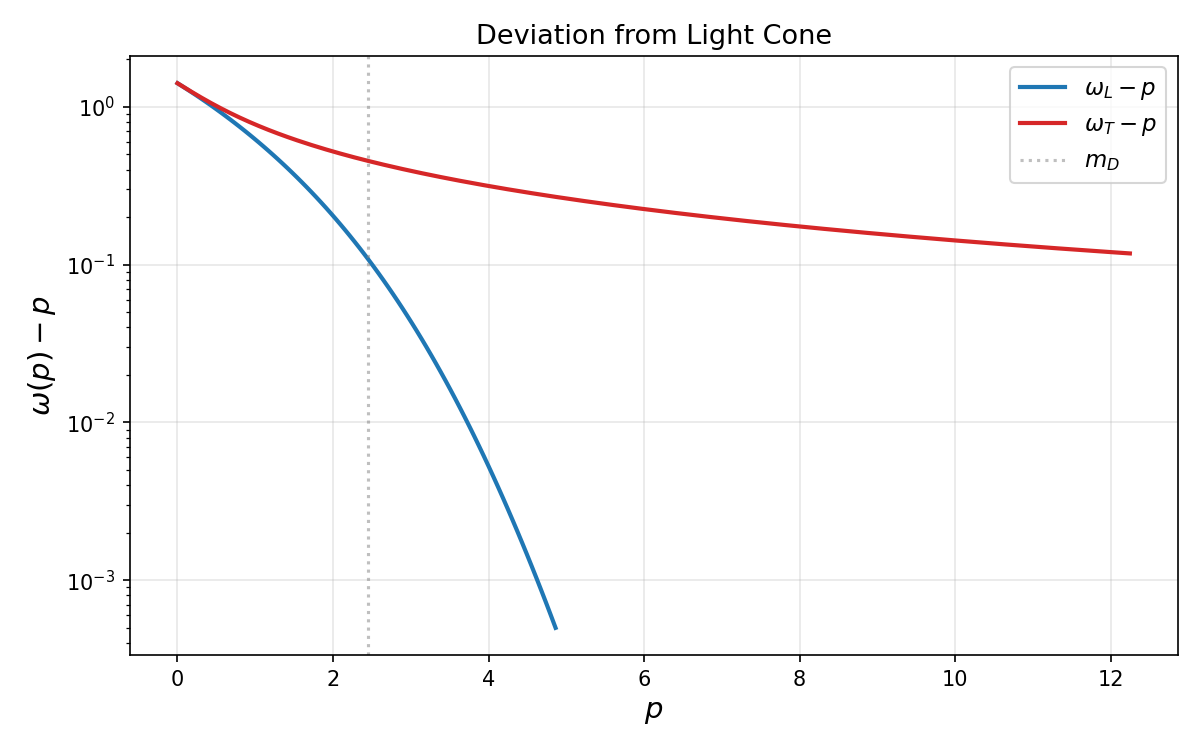
\includegraphics[width=0.85\textwidth]{03_HTL_asymptotic.png}
\caption{$\omega(p) - p$ 随动量的变化，展示纵横模式趋近光锥的不同方式。纵向模式指数衰减，横向模式幂律衰减。}
\label{fig:htl-asym}
\end{figure}

\begin{figure}[htbp]
\centering
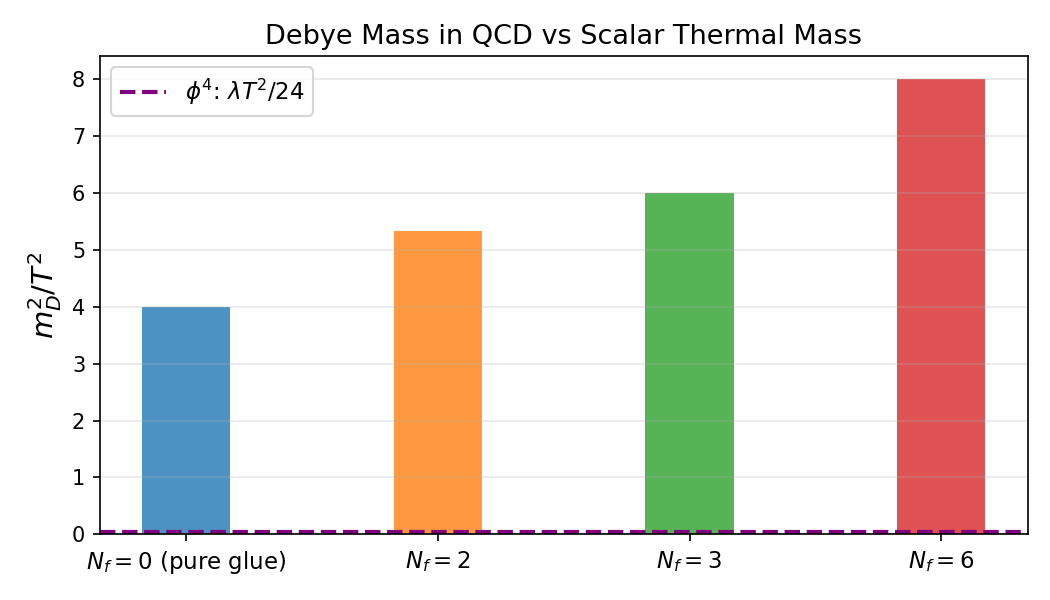
\includegraphics[width=0.85\textwidth]{03_mD_comparison.png}
\caption{QCD 德拜质量与 $\phi^4$ 热质量的比较。德拜质量 $m_D$ 是 QGP 中最基本的屏蔽尺度，直接控制着喷注淬火 $\hat q$ 和重夸克扩散系数 $\kappa$。}
\label{fig:mD-comp}
\end{figure}

\section{总结与展望}

本文展示了从有限温场论的基本公式出发，透过约 300 行 Python 代码，
完成从松原和到等离激元色散的完整计算。主要收获：

\begin{enumerate}[nosep]
\item 有限温度的微扰计算可自然地拆解为“解析推导”和“数值积分/求根”两步；
\item 热质量 $m_{\text{th}}^2$ 的数值结果在高温下精确趋近 $\lambda T^2/24$；
\item 谱函数从自由 $\delta$ 函数演化为高温下的 Breit-Wigner 形式，
反映了准粒子在热浴中获得有效质量与有限寿命的物理图像；
\item HTL 自能的数值求解揭示了 QGP 中等离激元的色散关系——在 $p=0$ 处简并为 $\omega_{\text{pl}} = m_D/\sqrt{3}$，
在 $p \to \infty$ 处趋近于光锥；
\item 以上所有结果均直接类比于 QGP 的德拜屏蔽、等离激元激发与夸克偶素溶解。
\end{enumerate}

\begin{thebibliography}{99}
\footnotesize
\bibitem{kapusta} J.~I.~Kapusta and C.~Gale,
\textit{Finite-Temperature Field Theory: Principles and Applications},
2nd ed. (Cambridge University Press, 2006).

\bibitem{laine} M.~Laine and A.~Vuorinen,
\textit{Basics of Thermal Field Theory},
Lect. Notes Phys. 925 (Springer, 2016).

\bibitem{lebellac} M.~Le~Bellac,
\textit{Thermal Field Theory} (Cambridge University Press, 1996).

\bibitem{mocsy} A.~Mócsy, P.~Petreczky, and M.~Strickland,
Quarkonium in medium: From correlation functions to PDFs,
\textit{Int. J. Mod. Phys. A} 28, 1340012 (2013).

\bibitem{rapps} R.~Rapp and H.~van~Hees,
Heavy quarks in the quark-gluon plasma, in
\textit{Quark-Gluon Plasma 4}, ed. R.~C.~Hwa and X.-N.~Wang
(World Scientific, 2010).

\bibitem{jeon} S.~Jeon,
Computing spectral densities in finite temperature field theory,
\textit{Phys. Rev. D} 47, 4586 (1993).

\bibitem{arnold} P.~Arnold, D.~T.~Son, and L.~G.~Yaffe,
Effective dynamics of hot, soft non-Abelian gauge fields,
\textit{Phys. Rev. D} 55, 6264 (1997).

\bibitem{majumder} A.~Majumder and M.~Van~Leeuwen,
The theory and phenomenology of perturbative QCD based jet quenching,
\textit{Prog. Part. Nucl. Phys.} 66, 41 (2011).

\bibitem{braaten} E.~Braaten and R.~D.~Pisarski,
Soft amplitudes in hot gauge theories: A general analysis,
\textit{Nucl. Phys. B} 337, 569 (1990).
\end{thebibliography}

\end{document}
